% Created by tikzDevice version 0.12.5 on 2023-12-06 02:46:58
% !TEX encoding = UTF-8 Unicode
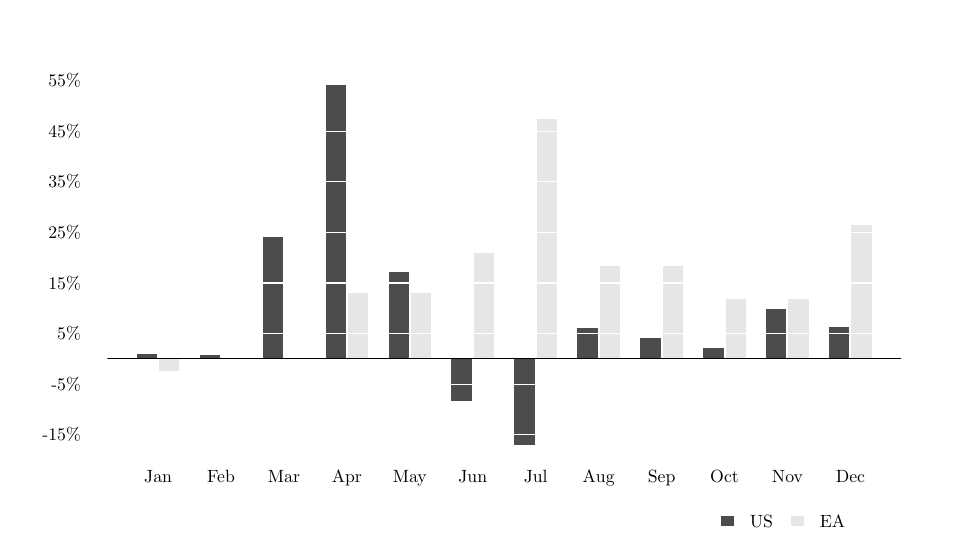
\begin{tikzpicture}[x=1pt,y=1pt]
\definecolor{fillColor}{RGB}{255,255,255}
\path[use as bounding box,fill=fillColor,fill opacity=0.00] (0,0) rectangle (325.21,180.67);
\begin{scope}
\path[clip] (  0.00,  0.00) rectangle (325.21,180.67);
\definecolor{fillColor}{gray}{0.30}

\path[fill=fillColor] ( 39.42, 61.00) rectangle ( 46.76, 62.66);
\definecolor{fillColor}{RGB}{230,230,230}

\path[fill=fillColor] ( 47.49, 61.00) rectangle ( 54.83, 56.73);
\definecolor{fillColor}{gray}{0.30}

\path[fill=fillColor] ( 62.16, 61.00) rectangle ( 69.50, 62.23);
\definecolor{fillColor}{RGB}{230,230,230}

\path[fill=fillColor] ( 70.23, 61.00) rectangle ( 77.57, 61.34);
\definecolor{fillColor}{gray}{0.30}

\path[fill=fillColor] ( 84.91, 61.00) rectangle ( 92.24,105.06);
\definecolor{fillColor}{RGB}{230,230,230}

\path[fill=fillColor] ( 92.98, 61.00) rectangle (100.31, 61.34);
\definecolor{fillColor}{gray}{0.30}

\path[fill=fillColor] (107.65, 61.00) rectangle (114.99,159.88);
\definecolor{fillColor}{RGB}{230,230,230}

\path[fill=fillColor] (115.72, 61.00) rectangle (123.06, 84.87);
\definecolor{fillColor}{gray}{0.30}

\path[fill=fillColor] (130.39, 61.00) rectangle (137.73, 92.31);
\definecolor{fillColor}{RGB}{230,230,230}

\path[fill=fillColor] (138.46, 61.00) rectangle (145.80, 84.87);
\definecolor{fillColor}{gray}{0.30}

\path[fill=fillColor] (153.13, 61.00) rectangle (160.47, 45.83);
\definecolor{fillColor}{RGB}{230,230,230}

\path[fill=fillColor] (161.20, 61.00) rectangle (168.54, 99.34);
\definecolor{fillColor}{gray}{0.30}

\path[fill=fillColor] (175.88, 61.00) rectangle (183.21, 30.01);
\definecolor{fillColor}{RGB}{230,230,230}

\path[fill=fillColor] (183.95, 61.00) rectangle (191.28,147.63);
\definecolor{fillColor}{gray}{0.30}

\path[fill=fillColor] (198.62, 61.00) rectangle (205.95, 72.01);
\definecolor{fillColor}{RGB}{230,230,230}

\path[fill=fillColor] (206.69, 61.00) rectangle (214.02, 94.70);
\definecolor{fillColor}{gray}{0.30}

\path[fill=fillColor] (221.36, 61.00) rectangle (228.70, 68.50);
\definecolor{fillColor}{RGB}{230,230,230}

\path[fill=fillColor] (229.43, 61.00) rectangle (236.77, 94.70);
\definecolor{fillColor}{gray}{0.30}

\path[fill=fillColor] (244.10, 61.00) rectangle (251.44, 64.79);
\definecolor{fillColor}{RGB}{230,230,230}

\path[fill=fillColor] (252.17, 61.00) rectangle (259.51, 82.67);
\definecolor{fillColor}{gray}{0.30}

\path[fill=fillColor] (266.84, 61.00) rectangle (274.18, 79.09);
\definecolor{fillColor}{RGB}{230,230,230}

\path[fill=fillColor] (274.91, 61.00) rectangle (282.25, 82.67);
\definecolor{fillColor}{gray}{0.30}

\path[fill=fillColor] (289.59, 61.00) rectangle (296.92, 72.67);
\definecolor{fillColor}{RGB}{230,230,230}

\path[fill=fillColor] (297.66, 61.00) rectangle (304.99,109.42);
\end{scope}
\begin{scope}
\path[clip] (  0.00,  0.00) rectangle (325.21,180.67);
\definecolor{drawColor}{RGB}{0,0,0}

\node[text=drawColor,anchor=base,inner sep=0pt, outer sep=0pt, scale=  0.64] at ( 47.13, 16.32) {Jan};

\node[text=drawColor,anchor=base,inner sep=0pt, outer sep=0pt, scale=  0.64] at ( 69.87, 16.32) {Feb};

\node[text=drawColor,anchor=base,inner sep=0pt, outer sep=0pt, scale=  0.64] at ( 92.61, 16.32) {Mar};

\node[text=drawColor,anchor=base,inner sep=0pt, outer sep=0pt, scale=  0.64] at (115.35, 16.32) {Apr};

\node[text=drawColor,anchor=base,inner sep=0pt, outer sep=0pt, scale=  0.64] at (138.09, 16.32) {May};

\node[text=drawColor,anchor=base,inner sep=0pt, outer sep=0pt, scale=  0.64] at (160.84, 16.32) {Jun};

\node[text=drawColor,anchor=base,inner sep=0pt, outer sep=0pt, scale=  0.64] at (183.58, 16.32) {Jul};

\node[text=drawColor,anchor=base,inner sep=0pt, outer sep=0pt, scale=  0.64] at (206.32, 16.32) {Aug};

\node[text=drawColor,anchor=base,inner sep=0pt, outer sep=0pt, scale=  0.64] at (229.06, 16.32) {Sep};

\node[text=drawColor,anchor=base,inner sep=0pt, outer sep=0pt, scale=  0.64] at (251.80, 16.32) {Oct};

\node[text=drawColor,anchor=base,inner sep=0pt, outer sep=0pt, scale=  0.64] at (274.55, 16.32) {Nov};

\node[text=drawColor,anchor=base,inner sep=0pt, outer sep=0pt, scale=  0.64] at (297.29, 16.32) {Dec};
\end{scope}
\begin{scope}
\path[clip] ( 28.80, 33.60) rectangle (315.62,161.47);
\definecolor{drawColor}{RGB}{0,0,0}

\path[draw=drawColor,line width= 0.4pt,line join=round,line cap=round] ( 28.80, 61.00) -- (315.62, 61.00);
\end{scope}
\begin{scope}
\path[clip] (  0.00,  0.00) rectangle (325.21,180.67);
\definecolor{drawColor}{RGB}{0,0,0}

\node[text=drawColor,anchor=base east,inner sep=0pt, outer sep=0pt, scale=  0.64] at ( 19.20, 31.40) {-15\%};

\node[text=drawColor,anchor=base east,inner sep=0pt, outer sep=0pt, scale=  0.64] at ( 19.20, 49.66) {-5\%};

\node[text=drawColor,anchor=base east,inner sep=0pt, outer sep=0pt, scale=  0.64] at ( 19.20, 67.93) {5\%};

\node[text=drawColor,anchor=base east,inner sep=0pt, outer sep=0pt, scale=  0.64] at ( 19.20, 86.20) {15\%};

\node[text=drawColor,anchor=base east,inner sep=0pt, outer sep=0pt, scale=  0.64] at ( 19.20,104.47) {25\%};

\node[text=drawColor,anchor=base east,inner sep=0pt, outer sep=0pt, scale=  0.64] at ( 19.20,122.74) {35\%};

\node[text=drawColor,anchor=base east,inner sep=0pt, outer sep=0pt, scale=  0.64] at ( 19.20,141.00) {45\%};

\node[text=drawColor,anchor=base east,inner sep=0pt, outer sep=0pt, scale=  0.64] at ( 19.20,159.27) {55\%};
\end{scope}
\begin{scope}
\path[clip] ( 28.80, 33.60) rectangle (315.62,161.47);
\definecolor{drawColor}{RGB}{255,255,255}

\path[draw=drawColor,line width= 0.4pt,line join=round,line cap=round] ( 28.80, 33.60) -- (315.62, 33.60);

\path[draw=drawColor,line width= 0.4pt,line join=round,line cap=round] ( 28.80, 51.87) -- (315.62, 51.87);

\path[draw=drawColor,line width= 0.4pt,line join=round,line cap=round] ( 28.80, 70.14) -- (315.62, 70.14);

\path[draw=drawColor,line width= 0.4pt,line join=round,line cap=round] ( 28.80, 88.40) -- (315.62, 88.40);

\path[draw=drawColor,line width= 0.4pt,line join=round,line cap=round] ( 28.80,106.67) -- (315.62,106.67);

\path[draw=drawColor,line width= 0.4pt,line join=round,line cap=round] ( 28.80,124.94) -- (315.62,124.94);

\path[draw=drawColor,line width= 0.4pt,line join=round,line cap=round] ( 28.80,143.21) -- (315.62,143.21);

\path[draw=drawColor,line width= 0.4pt,line join=round,line cap=round] ( 28.80,161.47) -- (315.62,161.47);
\end{scope}
\begin{scope}
\path[clip] (  0.00,  0.00) rectangle (325.21,180.67);
\definecolor{fillColor}{gray}{0.30}

\path[fill=fillColor, yshift = -12.5] (250.60, 16.88) rectangle (255.20, 13.04);
\definecolor{fillColor}{RGB}{230,230,230}

\path[fill=fillColor, yshift = -12.5] (275.88, 16.88) rectangle (280.48, 13.04);
\definecolor{drawColor}{RGB}{0,0,0}

\node[text=drawColor,anchor=base west,inner sep=0pt, outer sep=0pt, scale=  0.64, yshift = -20] at (260.96, 12.76) {US};

\node[text=drawColor,anchor=base west,inner sep=0pt, outer sep=0pt, scale=  0.64, yshift = -20] at (286.24, 12.76) {EA};
\end{scope}
\end{tikzpicture}
